\documentclass[12pt]{article}
\usepackage[fleqn]{amsmath}     %puts eqns to left, not centered
\usepackage{color}
\definecolor{light-gray}{gray}{0.15}
\definecolor{darker-gray}{gray}{0.05}
\usepackage{fancyvrb}
\usepackage{graphicx}
\usepackage{hyperref}
\usepackage{geometry}
\begin{document}
\section{Illustrations of numerical integration}

\subsection{Newton Cotes formulas and errors}


A Newton-Cotes formula uses an interpolating polynomial over $[a,b]$ to estimate $f$ and in turn the integral of $f$ over $[a,b]$. The nodes are evenly spaced, e.g.: \texttt{{a}}, \texttt{{a,b}}, \texttt{{a,(a+b)/2, b}}, ...

\begin{Verbatim}[framesep=1mm,frame=leftline,fontfamily=courier,formatcom=\color{darker-gray}]
linspace(a,b,n=251) = range(a,stop=b, length=n)
function interpolating_nodes(a, b, n)
  n == 0 && return [a]
  collect(linspace(a,b,n+1))
end

function l(i, nodes)
  length(nodes) == 1 && return(x -> 1.0)
  x -> begin
    prod((x-nodes[j])/(nodes[i]-nodes[j]) for j in eachindex(nodes) if i !== j)
  end
end

function poly_interp(f, nodes)
  x -> sum(f(nodes[i]) * l(i, nodes)(x) for i in eachindex(nodes))
end

function quadrature(f, a, b, nodes)
	As = [quadgk(l(i, nodes), a, b)[1] for i in eachindex(nodes)]
	sum(f(nodes[i]) * As[i] for i in eachindex(nodes))
end

function newton_cotes(f, a, b, n)
  nodes = interpolating_nodes(a, b, n)
  quadrature(f, a, b, nodes)
end
\end{Verbatim}
\begin{Verbatim}[framesep=3mm,frame=leftline, fontshape=it,formatcom=\color{darker-gray}]
newton_cotes (generic function with 1 method)
\end{Verbatim}
 
\begin{Verbatim}[framesep=1mm,frame=leftline,fontfamily=courier,formatcom=\color{darker-gray}]
using Plots, QuadGK
f = sin
a, b = 0, pi/2
plot(f, a, b)
plot!(poly_interp(f, interpolating_nodes(a, b, 0)), color=:red)
plot!(poly_interp(f, interpolating_nodes(a, b, 1)), color=:brown)
plot!(poly_interp(f, interpolating_nodes(a, b, 2)), color=:yellow)
\end{Verbatim}
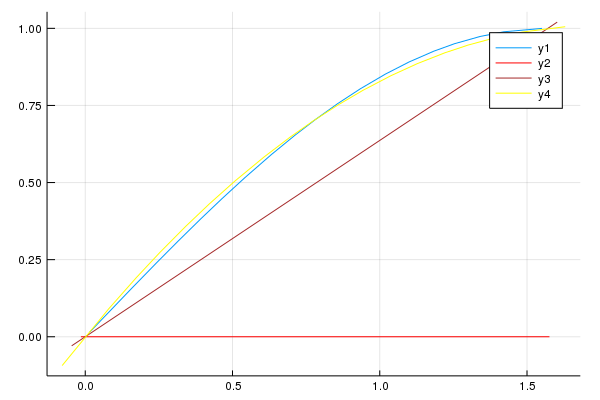
\includegraphics[width=0.65\textwidth]{fig-5-15380003412848600200.png}
 

How accurate for the sine function

\begin{Verbatim}[framesep=1mm,frame=leftline,fontfamily=courier,formatcom=\color{darker-gray}]
quadgk(f, a, b)  # 1.0
\end{Verbatim}
\begin{Verbatim}[framesep=3mm,frame=leftline, fontshape=it,formatcom=\color{darker-gray}]
(0.9999999999999999, 1.1102230246251565e-16)
\end{Verbatim}
 
\begin{Verbatim}[framesep=1mm,frame=leftline,fontfamily=courier,formatcom=\color{darker-gray}]
[newton_cotes(f, a, b, i) for i in 0:6] .- 1.0
\end{Verbatim}
\begin{Verbatim}[framesep=3mm,frame=leftline, fontshape=it,formatcom=\color{darker-gray}]
7-element Array{Float64,1}:
 -1.0                  
 -0.21460183660255172  
  0.0022798774922103693
  0.001004923314278816 
 -8.434527007272763e-6 
 -4.7386138333216365e-6
  2.5837235240189216e-8
\end{Verbatim}
 

Should be exact for polynomials of degree $n$ or less – but not necessarily more:

\begin{Verbatim}[framesep=1mm,frame=leftline,fontfamily=courier,formatcom=\color{darker-gray}]
a, b = 0, 1
function err(n)
  fn = x -> x^n  # x-> x^(n+1)
  nodes = interpolating_nodes(a, b, n)
  p = poly_interp(fn, nodes)
  newton_cotes(p, a, b, n) - quadgk(fn, a, b)[1]
end
[err(n) for n in 0:6]
\end{Verbatim}
\begin{Verbatim}[framesep=3mm,frame=leftline, fontshape=it,formatcom=\color{darker-gray}]
7-element Array{Float64,1}:
  0.0                   
  0.0                   
  5.551115123125783e-17 
  5.551115123125783e-17 
 -2.7755575615628914e-17
 -2.7755575615628914e-17
 -5.551115123125783e-17 
\end{Verbatim}
 
\subsection{Gauss quadrature}


Legendre polynomials satisfy $P_0=1$, $P_1(x) = x$, and $(n+1)P_{n+1}(x) = (2n+1)xP_n(x) -nP_{n-1}(x)$.

\begin{Verbatim}[framesep=1mm,frame=leftline,fontfamily=courier,formatcom=\color{darker-gray}]
using SymPy
@vars x
ps = Sym[1, x]
for n = 1:5
   pn, pn_1 = ps[end], ps[end-1]
   p =( (2n+1) * x*pn - n*pn_1 ) * (1// (n+1))
   push!(ps, simplify(p))
end
ps
\end{Verbatim}
\[ \left[ \begin{array}{r}1\\x\\\frac{3 x^{2}}{2} - \frac{1}{2}\\\frac{x \left(5 x^{2} - 3\right)}{2}\\\frac{35 x^{4}}{8} - \frac{15 x^{2}}{4} + \frac{3}{8}\\\frac{x \left(63 x^{4} - 70 x^{2} + 15\right)}{8}\\\frac{231 x^{6}}{16} - \frac{315 x^{4}}{16} + \frac{105 x^{2}}{16} - \frac{5}{16}\end{array} \right] \]
We were told these were \textit{orthogonal}:

\begin{Verbatim}[framesep=1mm,frame=leftline,fontfamily=courier,formatcom=\color{darker-gray}]
w = 1
[integrate(ps[i] * ps[j] * w, (x, -1, 1)) for i in eachindex(ps), j in eachindex(ps) if i < j]
\end{Verbatim}
\[ \left[ \begin{array}{r}0\\0\\0\\0\\0\\0\\0\\0\\0\\0\\0\\0\\0\\0\\0\\0\\0\\0\\0\\0\\0\end{array} \right] \]
We were told that these give exact quadrature for polynomials in $\Pi_{2n+1}$.

\begin{Verbatim}[framesep=1mm,frame=leftline,fontfamily=courier,formatcom=\color{darker-gray}]
n = 5
a,b = -1, 1
pn = ps[n+1]  # 1 - based
nodes = solve(pn)  # solve p(x) == 0
\end{Verbatim}
\[ \left[ \begin{array}{r}0\\- \sqrt{- \frac{2 \sqrt{70}}{63} + \frac{5}{9}}\\\sqrt{- \frac{2 \sqrt{70}}{63} + \frac{5}{9}}\\- \sqrt{\frac{2 \sqrt{70}}{63} + \frac{5}{9}}\\\sqrt{\frac{2 \sqrt{70}}{63} + \frac{5}{9}}\end{array} \right] \]\begin{Verbatim}[framesep=1mm,frame=leftline,fontfamily=courier,formatcom=\color{darker-gray}]
function err(i)
   fn = x -> x^i
   Fn = x -> x^(i+1)/(i+1)
   quadrature(fn, a, b, N.(nodes)) - (Fn(b) - Fn(a))
end
n = length(nodes) - 1
[err(i) for i in 0:2n+1]
\end{Verbatim}
\begin{Verbatim}[framesep=3mm,frame=leftline, fontshape=it,formatcom=\color{darker-gray}]
10-element Array{Float64,1}:
 -2.220446049250313e-16 
 -1.1102230246251565e-16
  0.0                   
 -5.551115123125783e-17 
  0.0                   
 -5.551115123125783e-17 
  0.0                   
 -5.551115123125783e-17 
  0.0                   
 -4.163336342344337e-17 
\end{Verbatim}
 

But 10th degree polys are not necessarily exact:

\begin{Verbatim}[framesep=1mm,frame=leftline,fontfamily=courier,formatcom=\color{darker-gray}]
fn = x -> x^10
Fn = x -> x^11/11
quadrature(fn, a, b, N.(nodes)) - (Fn(b) - Fn(a))
\end{Verbatim}
\begin{Verbatim}[framesep=3mm,frame=leftline, fontshape=it,formatcom=\color{darker-gray}]
-0.002931812455622018
\end{Verbatim}
 
\subsection{Error}


Thm 4 on p497 has: if $f$ is in $C^{2n}([a,b])$ where $g(x)$ is of degree $n$ (so that there are $n$ nodes) then (note $n-1$):


$$
E = \int_a^b f(x) w(x)dx - \sum_{i-1}^{n-1} f(x_i) A_i
= \frac{f^{(2n)}(\xi)}{(2n)!} \int_a^b q^2(x) w(x) dx
= \frac{f^{(2n)}(\xi)}{(2n)!} \langle q,q \rangle_w
$$



Here $q(x) = \Pi(x - x_i)$.


For this $n=5$ we have the exact integral

\begin{Verbatim}[framesep=1mm,frame=leftline,fontfamily=courier,formatcom=\color{darker-gray}]
q = prod(x-xi for xi in nodes)
integrate(q*q*w, (x, a, b))
\end{Verbatim}
\begin{equation*}\frac{128}{43659}\end{equation*}
So for $f(x) = x^{10}$  we have $f^{(10)}(\xi)/10! = 1$ and so the error is

\begin{Verbatim}[framesep=1mm,frame=leftline,fontfamily=courier,formatcom=\color{darker-gray}]
float(integrate(q*q*w, (x, a, b)))
\end{Verbatim}
\begin{Verbatim}[framesep=3mm,frame=leftline, fontshape=it,formatcom=\color{darker-gray}]
0.0029318124556219796
\end{Verbatim}
 

Which matches what was previously found.

\subsubsection{Simpson's error}


If we used 5 points and simpson's formula, then we would apply simpsons over $x_0, x_1, x_2$ and $x_2, x_3, x_4$. How accurate would that be?

\begin{Verbatim}[framesep=1mm,frame=leftline,fontfamily=courier,formatcom=\color{darker-gray}]
nodes = N.(nodes) # make floating point
quadrature(fn, nodes[1], nodes[3], nodes[1:3]) +
quadrature(fn, nodes[3], nodes[5], nodes[3:5]) - (Fn(1) - Fn(-1))
\end{Verbatim}
\begin{Verbatim}[framesep=3mm,frame=leftline, fontshape=it,formatcom=\color{darker-gray}]
-0.118219124196878
\end{Verbatim}
 

So quite far off by comparison

\subsection{QuadGk}


The \href{https://github.com/JuliaMath/QuadGK.jl}{QuadGK} package, as seen, performs integration. The name is now less opaque:

\begin{enumerate}\item 
\texttt{Quad} as we are performing quadrature\item 
\texttt{G} For Guass\item 
\texttt{K} is for Kronrod, who added a computationally important step\end{enumerate}


The basic idea is to adaptively integrate over a region using Gaussian quadrature. If the estimated error in a region is too large, the region is split in two and Gaussian quadrature is used to investigate each piece. The method is quite efficient.


For example, with errors like $1/n$, $1/n^2$ and $1/n^4$ for Riemann, Trapezoid and Simpsons, we see that it might take 10^4 steps to get machine tolerance accuracy.


For example, to integrate $\sin(x)$ over $[0, \pi]$ using Simpson's we have

\begin{Verbatim}[framesep=1mm,frame=leftline,fontfamily=courier,formatcom=\color{darker-gray}]
simpson(f, a, b) = 1/6 * (f(a) + 4f((a+b)/2) + f(b))
a, b = 0, pi
n = 10_000
xs = linspace(a, b, n)
sum(simpson(sin, a, b)*(b-a) for (a,b) in zip(xs[1:end-1], xs[2:end])) - 2.0
\end{Verbatim}
\begin{Verbatim}[framesep=3mm,frame=leftline, fontshape=it,formatcom=\color{darker-gray}]
-1.1102230246251565e-15
\end{Verbatim}
 

How many function calls is this?

\begin{Verbatim}[framesep=1mm,frame=leftline,fontfamily=courier,formatcom=\color{darker-gray}]
mutable struct CountingFunction
  n::Int
  f::Function
  CountingFunction(f) = new(0, f)
end
(F::CountingFunction)(x) = (F.n += 1; F.f(x))
\end{Verbatim}

And

\begin{Verbatim}[framesep=1mm,frame=leftline,fontfamily=courier,formatcom=\color{darker-gray}]
Sin = CountingFunction(sin)
sum(simpson(Sin, a, b)*(b-a) for (a,b) in zip(xs[1:end-1], xs[2:end])) - 2.0
\end{Verbatim}
\begin{Verbatim}[framesep=3mm,frame=leftline, fontshape=it,formatcom=\color{darker-gray}]
-1.1102230246251565e-15
\end{Verbatim}
 

How many steps:

\begin{Verbatim}[framesep=1mm,frame=leftline,fontfamily=courier,formatcom=\color{darker-gray}]
Sin.n
\end{Verbatim}
\begin{Verbatim}[framesep=3mm,frame=leftline, fontshape=it,formatcom=\color{darker-gray}]
29997
\end{Verbatim}
 

Whereas for \texttt{quadgk}:

\begin{Verbatim}[framesep=1mm,frame=leftline,fontfamily=courier,formatcom=\color{darker-gray}]
Sin = CountingFunction(sin)
quadgk(Sin, 0, pi)
\end{Verbatim}
\begin{Verbatim}[framesep=3mm,frame=leftline, fontshape=it,formatcom=\color{darker-gray}]
(2.0, 1.7905676941154525e-12)
\end{Verbatim}
 

and

\begin{Verbatim}[framesep=1mm,frame=leftline,fontfamily=courier,formatcom=\color{darker-gray}]
Sin.n
\end{Verbatim}
\begin{Verbatim}[framesep=3mm,frame=leftline, fontshape=it,formatcom=\color{darker-gray}]
15
\end{Verbatim}
 

\end{document}
